\input{../preamble.tex}

\lecturenumber{1}
\title{Intro To Operating\\Systems}
\version{2.0.1}

\begin{document}

\begin{frame}[plain, noframenumbering]
    \titlepage
\end{frame}

\begin{slide}

	\slidetitle{About Me: My name is Talia}
	
	\vspace{-5mm}
	
	\begin{minipage}[t]{0.25\textwidth}
        \vspace{0pt}\par
		\vspace{7mm}
        
\includegraphics[width=25mm]{talia-xu.jpeg}
    \end{minipage}
    \hfill
    \begin{minipage}[t]{0.7\textwidth}
        \vspace{0pt}\par
        
        \textbf{Lecturer}
		
		\leftspace Computer Science
        \medskip
		
        \textbf{Research Interest:}
		
		\leftspace Embedded Systems, 
		
		\leftspace Low Power Wireless Communication, 
		
		\leftspace IoT / Batteryless Systems.
        \bigskip
		
        I mostly teach \textbf{systems courses}, 
		
		\leftspace operating systems, computer organization, etc.
        
    \end{minipage}
	
\end{slide}

\begin{slide}

	\slidetitle{Agenda}

	About the course
	\bigskip
	
	Introduction to Operating Systems
	\bigskip
	
	First topic: Process
	
\end{slide}

\begin{slide}

	\slidetitle{Lecture Times and Location}
	
	\begin{tabular}{l l l}
		Mon: & 1pm - 2pm & 303-G02 \\
		Tues: & 1pm - 2pm & 405-460 \\
		Wed: & 1pm - 2pm & 106-204 \\
	\end{tabular}
	
	\bigskip
	
	\textbf{Lecture Slides}: Generally available by the end of the day before each lecture.
	
	\medskip
	
	\textbf{Lecture Recordings}: Posted by the end of the day of the lecture.
	
	\medskip
	
	\textbf{Practice Questions}: Lectures will include practice questions similar to those you will see on the test and final exam.
	
	\medskip
	
	\textbf{Interactive Quizzes}: Any interactive quizzes used in class will not be posted separately, but you can review them in the lecture recordings.
	
\end{slide}

\begin{slide}

    \slidetitle{Your Instructors}
  
        \textbf{Talia Xu}
                
        \leftspace Instructor: Week 1 - 6
        
        \leftspace Office: 303S-592
        
        \leftspace Email: talia.xu@auckland.ac.nz
        
		\leftspace Office hour: by appointment
    
    \bigskip
    
        \textbf{Shyamli Sindhwani}
        
        (Course Director/Coordinator)
        
        \leftspace Instructor: Week 7 - 12
        
        \leftspace Office: 303-409
        
        \leftspace Email: shyamli.sindhwani@auckland.ac.nz
        
		\leftspace Office hour: by appointment
  
\end{slide}

\begin{slide}

    \slidetitle{Tutorial: Wed 3pm - 4pm 303-G01}

	\textbf{Zhihang Liu}

	Email: zliu604@aucklanduni.ac.nz

	\medskip

	\textbf{Steve Le}

	Email: qle752@aucklanduni.ac.nz
	
	\bigskip
	
	\textbf{Format}: Tutorials are a mix of reviews of course content, practice questions, and help sessions for assignments.

	\medskip

	\textbf{Resources}: Tutorials are not recorded, but slides will be shared before each tutorial.

	\medskip

	\textbf{Assignments}: TAs are also responsible for marking assignments. Please direct your assignment-related inquiries to them.

\end{slide}

\begin{slide}

    \slidetitle{Evaluation for this course}
    
    \begin{center}
        \begin{tabular}{  l l l l  } 
          \textbf{Assessment} & \textbf{Weight} & \textbf{Due Date} \\ 
          Assignment 1 & 10\% & April 3 \\ 
          Midterm & 20\% & April 21 @ 6:30 pm \\ 
          Assignment 2 & 10\% & May 8 \\ 
          Assignment 3 & 10\% & May 29  \\ 
          Final & 50\% & TBD \\ 
        \end{tabular}
    \end{center}
	
	\medskip
		
	\textbf{Overall Mark}: To pass the course, you must achieve at least 50\% for your overall course mark.
	
	\medskip
	
	\textbf{Test/Exam Component}: You must also pass the combined test/exam component. This test/exam component is worth 70\% of the overall mark, consisting of the test (worth 20\%) and the final exam (worth 50\%). To pass this component, you need to get at least 35 out of 70.    
		
\end{slide}

\begin{slide}
  
    \slidetitle{Aegrotat / Compassionate Consideration Policy}

    If circumstances impacted your ability to sit an invigilated assessment, or impaired your preparation/performance, we will organise an alternative assessment. 
	
	\medskip
	
	The alternative assessment may be in the same format or in an alternative format such as viva voce/oral test.
  
\end{slide}

\begin{slide}
  
    \slidetitle{The Recommended Books Complement Lectures}

    ``\href{https://pages.cs.wisc.edu/~remzi/OSTEP/}
           {Operating Systems: Three Easy Pieces}'' \\
    by \href{http://www.cs.wisc.edu/~remzi/}{Remzi Arpaci-Dusseau}
    and \href{http://www.cs.wisc.edu/~dusseau/}{Andrea Arpaci-Dusseau}
    \bigskip

    ``\href{https://www.wiley.com/en-ie/Silberschatz's+Operating+System+Concepts%2C+Global+Edition%2C+10th+Edition-p-9781119454083}
            {Silberschatz's Operating System Concepts, 10th Edition, Global Edition}'' \\
    by \href{https://seas.yale.edu/faculty-research/faculty-directory/abraham-silberschatz}{Abraham Silberschatz} 
    and \href{https://dl.acm.org/profile/81100611528}{Peter B. Galvin}
    and \href{https://greggagne.github.io/}{Greg Gagne}
    \bigskip
    
    ``\href{https://en.wikipedia.org/wiki/The_C_Programming_Language}
           {The C Programming Language}'' \\
    by \href{https://en.wikipedia.org/wiki/Brian_Kernighan}{Brian Kernighan}
    and \href{https://en.wikipedia.org/wiki/Dennis_Ritchie}{Dennis Ritchie}

\end{slide}

\begin{slide}
  
    \slidetitle{Skills You Should Practice Again If Needed}

    Programming
    \begin{itemize}
        \item C Programming and Debugging
        \item Python Programming and Debugging
    \end{itemize}
    
    \bigskip

    Basic Concepts
    \begin{itemize}
        \item Being able to convert between binary, hex, and decimal
        \item Memory being byte-addressable, memory addresses (pointers)
    \end{itemize}
        
\end{slide}

\begin{slide}
  
    \slidetitle{Why Operating Systems?}

    Understanding the operating system will make you a better programmer
    \bigskip

    You will either write software that:
    \begin{itemize}
        \item Interacts with the operating system
        \item Is the operating system
    \end{itemize}
  
    \bigskip
    
    Not always important if you only care about functionality.
    \medskip
    
    Important when performance matters in your program.
    
\end{slide}

\begin{slide}

    \slidetitle{Why Operating Systems?}
    
    \begin{minted}{c}
int array[ROWS][COLS];
for (int i = 0; i < ROWS; i++) {
    for (int j = 0; j < COLS; j++) {
        array[i][j] = i * COLS + j;
    }
}
    \end{minted}   
	
	\bigskip
	
	\begin{minted}{c}
int array[ROWS][COLS];
for (int j = 0; j < COLS; j++) {
    for (int i = 0; i < ROWS; i++) {
        array[i][j] = i * COLS + j;
    }
}
	\end{minted}    
    
\end{slide}

\begin{slide}

    \slidetitle{Why Operating Systems?}

\begin{minted}{c}
// 1 + 2 + 3 + 4 + 5 + ... + n = 100

int  iterative_addition(int  n) {
    int  sum = 0;
    for (int  i = 0; i < n; i++) {
        sum += i;
    }
    return sum;
}

int  recursive_addition(int  n) {
    if (n == 0) return 0;
    return (n - 1) + recursive_addition(n - 1);
}
\end{minted}
    
\end{slide}

\begin{slide}
  
	\slidetitle{An Operating System Manages Resources}

	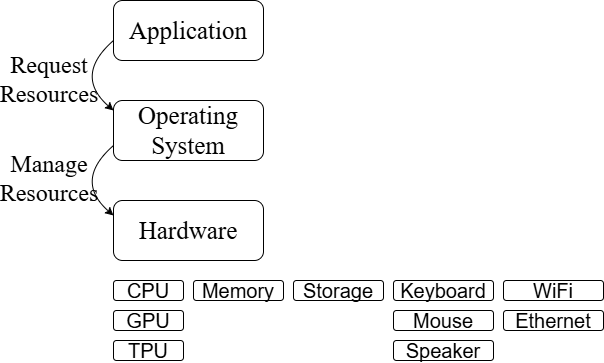
\includegraphics[width=75mm]{operating-system-overview.png}

\end{slide}

\begin{slide}

	\slidetitle{We have all used multiple OS}
	
	Windows
	
	Linux
	
	MacOS
	
	Android 
	
	IOS
	
	ChromeOS
	
	....
	
	\bigskip
	
	Are they just the same OS with different names?
	
	\medskip
	
	How are they different?

\end{slide}

\begin{slide}
  
	\slidetitle{Three Core Operating System Concepts}

	\textbf{Virtualization} 
	
	\leftspace lets each program think it has the whole computer to itself

	\bigskip

	\textbf{Concurrency} 
	
	\leftspace allows multiple tasks to appear to happen at once
	
	\bigskip

	\textbf{Persistence} 
	
	\leftspace guarantees that data will stick around and can be retrieved later
  
\end{slide}

\begin{slide}
  
	\slidetitle{Our First Abstraction is a Process}

	\textbf{Program:} a file containing all the instructions and data required to run
	\bigskip

	\textbf{Process:} an instance of running a program
  
\end{slide}

\begin{slide}
  
	\slidetitle{The Basic Requirements for a Process}

	How are you able to run two different programs at the same time?
	\bigskip

	For example, a ``hello world'' program and another that counts up one every second
	
	\vspace{-15mm}
	
	\centering
	
\includegraphics{process-basic.eps}

\end{slide}

\begin{slide}
  
	\slidetitle{Potential Memory Layout for Multiple Processes}

	\centering

	\includegraphics<1>{memory-layout-first.eps}%
	\includegraphics<2>{memory-layout-second.eps}
  
\end{slide}

\begin{slide}
  
	\slidetitle{What Happens If Two Processes Run the Same Program?}

	\inputminted{c}{count.c}

\end{slide}

\begin{slide}
  
	\slidetitle{What Did We Find?}

	Was the address of \mintinline{c}{local} the same between the two processes?
	\medskip

	Was the address of \mintinline{c}{global} the same between the two processes?
	\medskip

	What else may be needed for a process?
  
\end{slide}

\begin{slide}
  
	\slidetitle{A Process Has Its Own Virtual Memory}

	\centering

	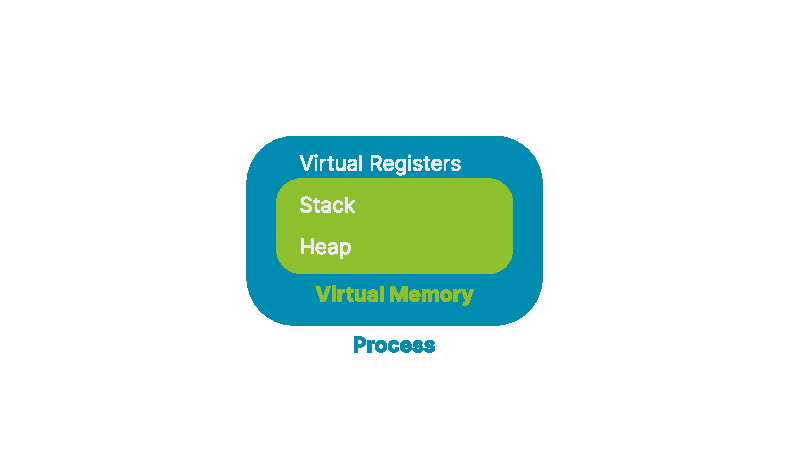
\includegraphics{process-virtual-memory.eps}

\end{slide}

\end{document}
